\chapter{Contribution \& Discussion}
\renewcommand{\thesection}{\arabic{section}}
		




\label{chapitre4}
		
		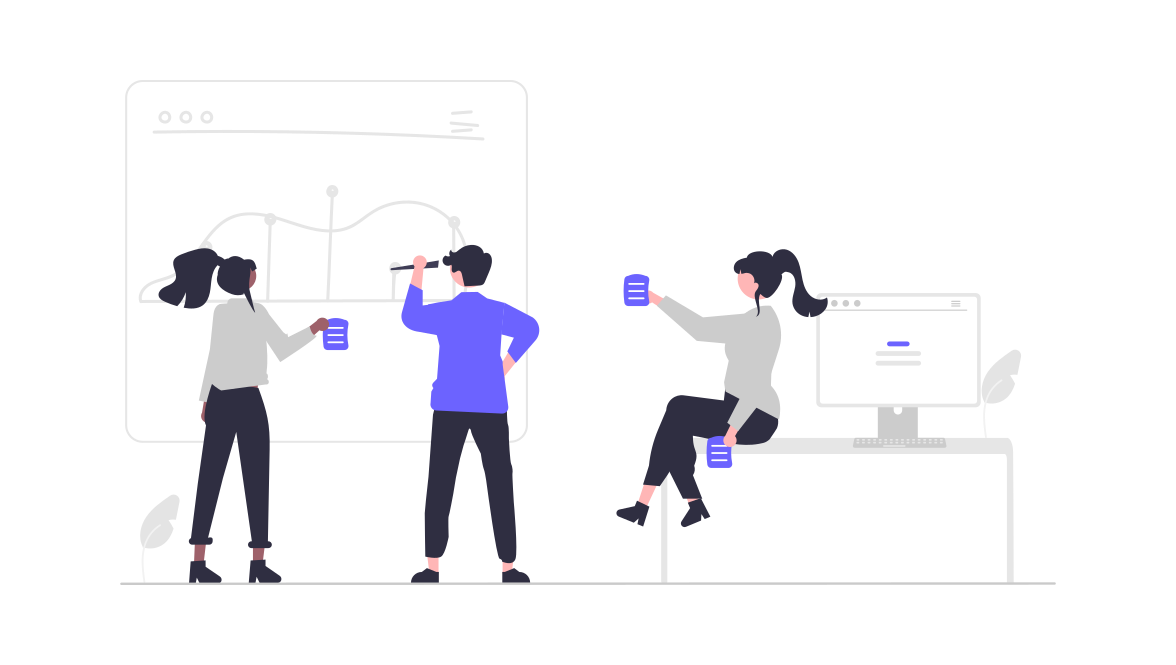
\includegraphics [width=1 \linewidth, height=0.8\textheight, keepaspectratio] {images/chaptersFigures/contribution.png}
		
	
		
    \newpage
    \thispagestyle{plain}

In this chapter, we propose our data management and visualization system for medical data that aims to manage the uncommon data from the various sources then provides a personalized dashboard for each actor based on their predefined needs.




\section{Work Objectives}
The aim of this work is to propose a system that organizes data coming from different sources then structures it in a way that enables easily to visualize it in most convenient ways (both useful and easy to read) for each actor. We are interested in the step between Rendering and Data image in the pipeline process(\ref{fig:infovispipeline}). After reviewing and analyzing similar proposed works, we created our own visualization system that will be detailed in the coming sections.



\section{Literature \& Related works review}
We present in this section architecture for healthcare data management systems, data warehouses and solutions that attempt to integrate infoVis into medical data and medical structures, which could be used by executive managers, doctors, physicians and other health professionals to support the healthcare process.  Medical data existing today in multiple sources with different formats makes it necessary to have certain data integration techniques. A healthcare data warehouse is therefore needed to integrate the different data sources into a central data repository and analyze this data.
\bigbreak

\begin{itemize}
  \renewcommand{\labelitemi}{$\bullet$}
  \item \textbf{\textit{A Healthcare Data Warehouse for Cancer Diseases:}} Dr.Osama E.Sheta and Ahmed Nour Eldeen discussed in their paper\cite{shetaBuildingHealthCare2012} the implementation of a healthcare data warehouse for cancer diseases, they proposed  two stages approach for the building cancer data warehouse: \bigbreak
  
  \begin{enumerate}
    
    \item \textit{Business Analysis:} Consist of business process analysis and business requirement analysis (Figure\ref{fig:cancerDiagrame}). \newpage
    \begin{figure}[h!]
      \center
      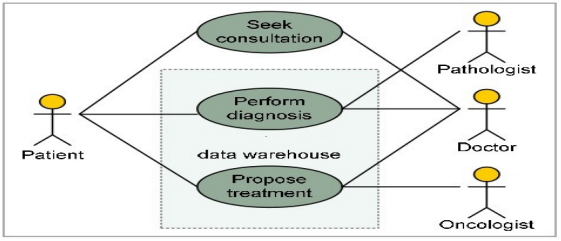
\includegraphics[width=0.75\textwidth]{images/chapter3/relatedwork/cancerDiagrame.PNG}
      \caption{Cancer data warehouse use case diagram.}
      \label{fig:cancerDiagrame}
    \end{figure}
    \item \textit{Architecture Design:} Data is imported from several sources and transformed within a staging area before it is integrated and stored in the production data warehouse for further analysis (Figure\ref{fig:cancersystem}).
     \begin{figure}[h!]
      \center
      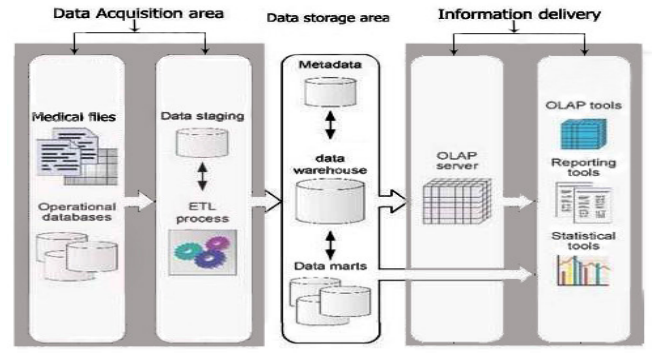
\includegraphics[width=0.90\textwidth]{images/chapter3/relatedwork/cancersystem.PNG}
      \caption{Cancer data warehouse Architecture Taken from the source.}
      \label{fig:cancersystem}
    \end{figure}
    \end{enumerate}
    \newpage
    \item \textbf{\textit{Data Warehouse Framework in Pharmaceutical Sector:}} In this paper\cite{abd2019proposed} authors proposed a data warehouse framework to enhance decisions of distribution systems in pharmaceutical companies to decrease the medicine industry cost and increase productivity. The framework can be described in four phases shown in (Figure \ref{fig:pharmacysystem}). Phase one consists of a data preparation, a phase which has four steps (data collection, building DBs, DWH and data cleaning). Phase two consists of training the data which is applying time series to three types of Neural Networks techniques (levenberg marquardt, Bayesian regularized, and Scaled conjugate gradient). Phase three is testing the performance based on mean square error (MSE). Phase four consists of evaluating the performance of the best prediction model.
    \begin{figure}[h!]
      \center
      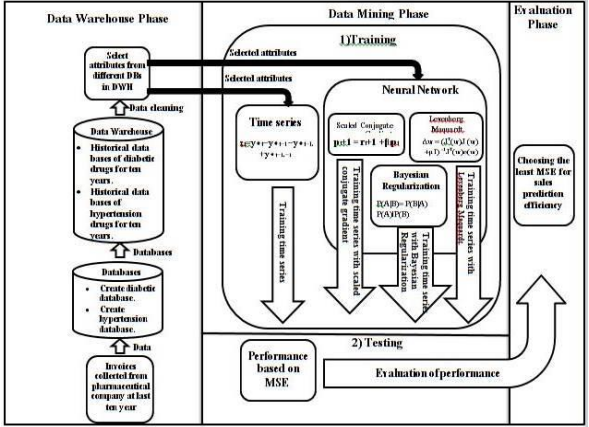
\includegraphics[width=0.80\textwidth]{images/chapter3/relatedwork/pharmacysystem.PNG}
      \caption{The Proposed Framework of Sales Prediction.}
      \label{fig:pharmacysystem}
    \end{figure}
    \newpage
    
    \item \textbf{\textit{Big Bata Warehouse Based On Hadoop Architecture:}} In this paper\cite{sebaa2018medical} entitled “Medical Big Data Warehouse: Architecture and System Design, a Case Study: Improving Healthcare Resources Distribution” authors proposed a system architecture and a conceptual data model for a MBDW (Medical Big Data Warehouse), and then offer a solution to overcome both the growing of fact table size and the lack of primary and foreign keys in the framework Apache Hive required in the conceptual data model. This solution is based on nested partitioning according to the dimension tables keys, then  applying their solution to implement a MBDW to improve medical resources distribution for the health sector in the Bejaia region (in Algeria). 
    \bigbreak
    The overall architecture is depicted in (Figure \ref{fig:bigdatarelated}). It is a scalable, reliable, and distributed architecture to extract, store, analyze, and visualize healthcare data extracted from various resources HIS (Hospitals Information systems).
    \begin{figure}[h!]
      \center
      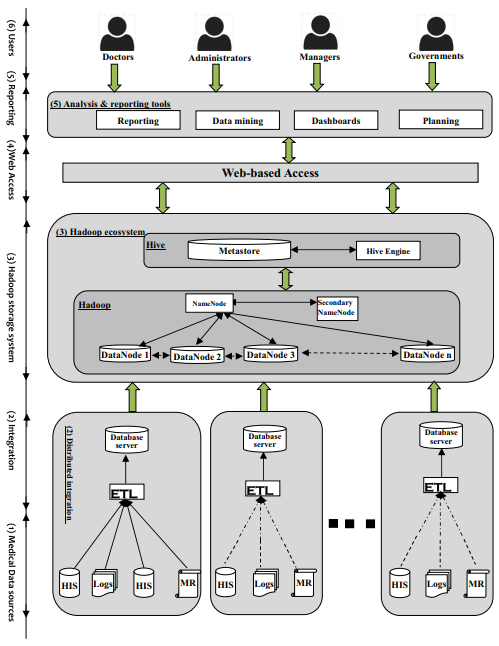
\includegraphics[width=0.60\textwidth]{images/chapter3/relatedwork/relatedworkHadoop.PNG}
      \caption{Hadoop-based system architecture of medical big data warehousing.}
      \label{fig:bigdatarelated}
    \end{figure}
\end{itemize}

\newpage
\section{Proposed Solution}
As mentioned in the project description, the presence of a visualization presentation in the medical sector is necessary. The proposed solution was to create a data management and visualization system that organizes and structures the data coming from various sources, then produces focus data in the eXtensible Markup Language (XML) format, this focus data will be visualized based on each actor and their preferend needs.\\
We mainly focused on the "Rendering" step in the visualization pipeline(\ref{fig:infovispipeline}), and we worked on the medical data type that are mentioned in the Table\ref{tab:sourceTable}.


\section{Why XML?}
The rise of XML (eXtensible Markup Language) in patient care has been driven by the needs for communication among health professionals and between healthcare organizations such as hospitals and health insurance companies.The main advantage of XML is its flexibility, as it allows creators to describe any content easily by generating their own tags\cite{thuy2012s}. Some of XML’s features are\cite{achard2001xml}:
\begin{itemize}
\renewcommand{\labelitemi}{$\bullet$}
\item The XML and DTD files are human readable and thus can be easily edited by people with only a few computer skills. Updating a data model is, therefore, straightforward (at least from a technical point of view).
\item XML is Internet-oriented and has very rich capabilities for linking data; this can be used for interconnecting databases.
\item XML provides an open framework for defining standard specifications. This is an important point because medical informatics clearly lacks standardization. For example, querying on multiple molecular biology databases could be greatly facilitated if each database would offer an XML view of their content.
\end{itemize}
On the other hand, XML has some weaknesses:
\begin{itemize}
\renewcommand{\labelitemi}{$\bullet$}
\item The overhead of a text based format in data parsing, storage and transmission needs to be evaluated before adopting XML as a general solution. However, a text format means that the source code can be read and edited with any text editor.
\item It is not clear whether XML satisfactorily addresses the problems of technological scalability. Indeed if XML data are stored in flat files, queries on XML files will not scale because XML in itself does not provide scalable facilities such as indexing or data clustering. This means that parsing should be done on the fly which leads to poor performances. One solution could be to have query optimizations done externally for example using a Database Management System (DBMS).
\end{itemize}
\bigbreak
At this point the question to be answered is whether the pros prevail over the cons, for this reason Frederic Achard and al\cite{achard2001xml}  have provided a comparison between XML and some of the most popular solutions that are used for the management and exchange of bioinformatics data summarized in the (Table\ref{tab:xmlcomparaison}), each one is rated with one to four stars for different criteria: the higher the number of stars, the better the solution with regard to the criteria.
\begin{table}[h!]
    \centering
    \begin{tabular}{|m{0.20\linewidth}|m{0.10\linewidth}|m{0.10\linewidth}|m{0.10\linewidth}|m{0.11\linewidth}|m{0.10\linewidth}|m{0.10\linewidth}|}
        \hline

        \textbf{Criteria}                      & \textbf{XML}        & \textbf{{\small Field/ value} }        & \textbf{{\small \gls{asn}}}    & \textbf{{\small \gls{cobra}}} &\textbf{{\small \gls{java}}}      & \textbf{{\small \gls{oodbms}}}      \\

        \hline
        Model expressiveness 	& **	& *		& *** & *** & *** & ****     \\
        
        \hline
        Constraints	    & **	& *	& *    & **   & ***   & ****       \\
        
        \hline
        Self-descriptive    & yes	& no	& yes    & yes   &  yes  &  yes      \\
        
        \hline
        Query language	 & soon 	& no	& no    & soon    & no   &  yes \\
        
        \hline
        Flexibility	 & ****	& *	& ***    &  ***  & ***   & ****  \\
        
        \hline
        Simplicity 	 & ****	& ****	& ***    & *   & **   & **  \\
        
        \hline
        Scalability 	 & **	& *	& **   & ***   & ***   & ****  \\
        
        \hline
        Interoperability 	 & ****	& *	&  **  & ****   & ****   & ***  \\
                
        \hline
    \end{tabular} 

    \caption{Summary of comparison of different alternatives to XML.}
    \label{tab:xmlcomparaison}
\end{table}
\bigbreak
They conclude that the use of XML as an intermediate medium would be really efficient only if all databases share common or very similar DTDs. Whatever language is used, it is always difficult to find an agreement on a common semantics, and when one is found, it is often revised. However, XML would be an excellent candidate for this role because of its flexibility.

\newpage

\section{The Proposed System Process}
Our system process is divided into three main phases as illustrated in the following figure. In this part, we will explain in detail the steps of each phase. 
\begin{figure}[h!]
  \center
  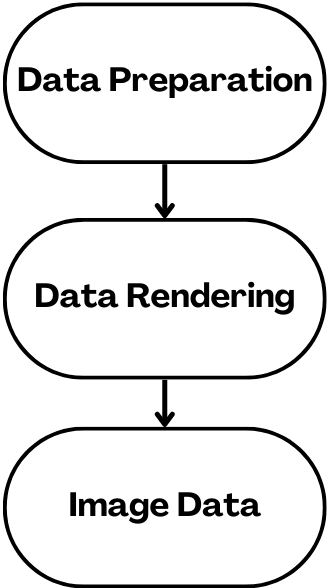
\includegraphics[width=0.20\textwidth]{images/chapter3/systemProcesss.png}
  \caption{The proposed system architecture.}
  \label{fig:system}
\end{figure}

\subsection{The Data Preparation}
It consists of 4 stages: The Data Collection, pretreatment, Data Integration \& Treatment, and output data as illustrated in the following figure. 
\begin{figure}[h!]
  \center
  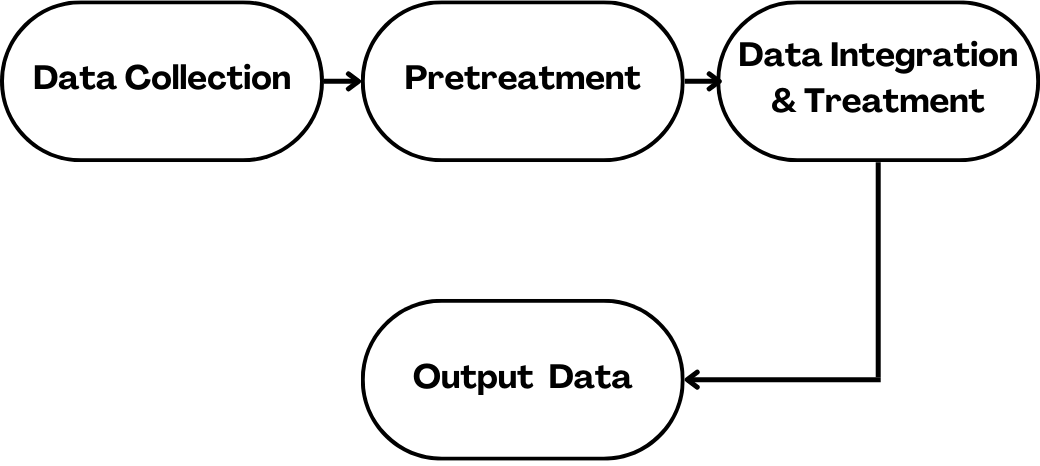
\includegraphics[width=0.60\textwidth]{images/chapter3/system.png}
  \caption{The Data preparation flowchart.}
  \label{fig:dataprep}
\end{figure}

\subsubsection*{The Data Collection}
The datasets chosen for this work come from kaggle\cite{KaggleYourHome}. Kaggle is an online community of data scientists and machine learning practitioners\cite{Kaggle2022}, it enables users to find and publish datasets, explore and build models in a data science environment based on the web, etc.\\
For the purposes of the creation process, we collected the following data (each is between 100K and 240K line) in csv format:
\begin{itemize}
  \renewcommand{\labelitemi}{$\bullet$}
  \item \textbf{Drugs Prescriptions with Providers Profile Dataset: }It contains recommended drugs based on medical practitioners  practicing specialty, years of practicing and previous suggested drugs in prescriptions by other providers or practitioners (Figure\ref{fig:drugs}).
  
  \begin{figure}[h!]
    \center
    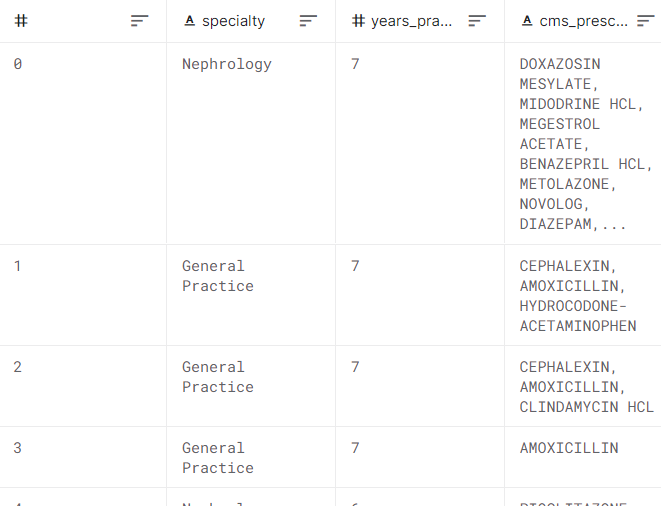
\includegraphics[width=0.50\textwidth]{images/chapter3/dataset/medicine_prescription_records - Copie.PNG}
    \caption{A sample of Drugs prescriptions dataset.}
    \label{fig:drugs}
  \end{figure}
 
   \item \textbf{Health Prescription Dataset: }It contains the patient's diagnosis, the admission type and the dates related (Figure\ref{fig:presc}).
   \begin{figure}[h!]
    \center
    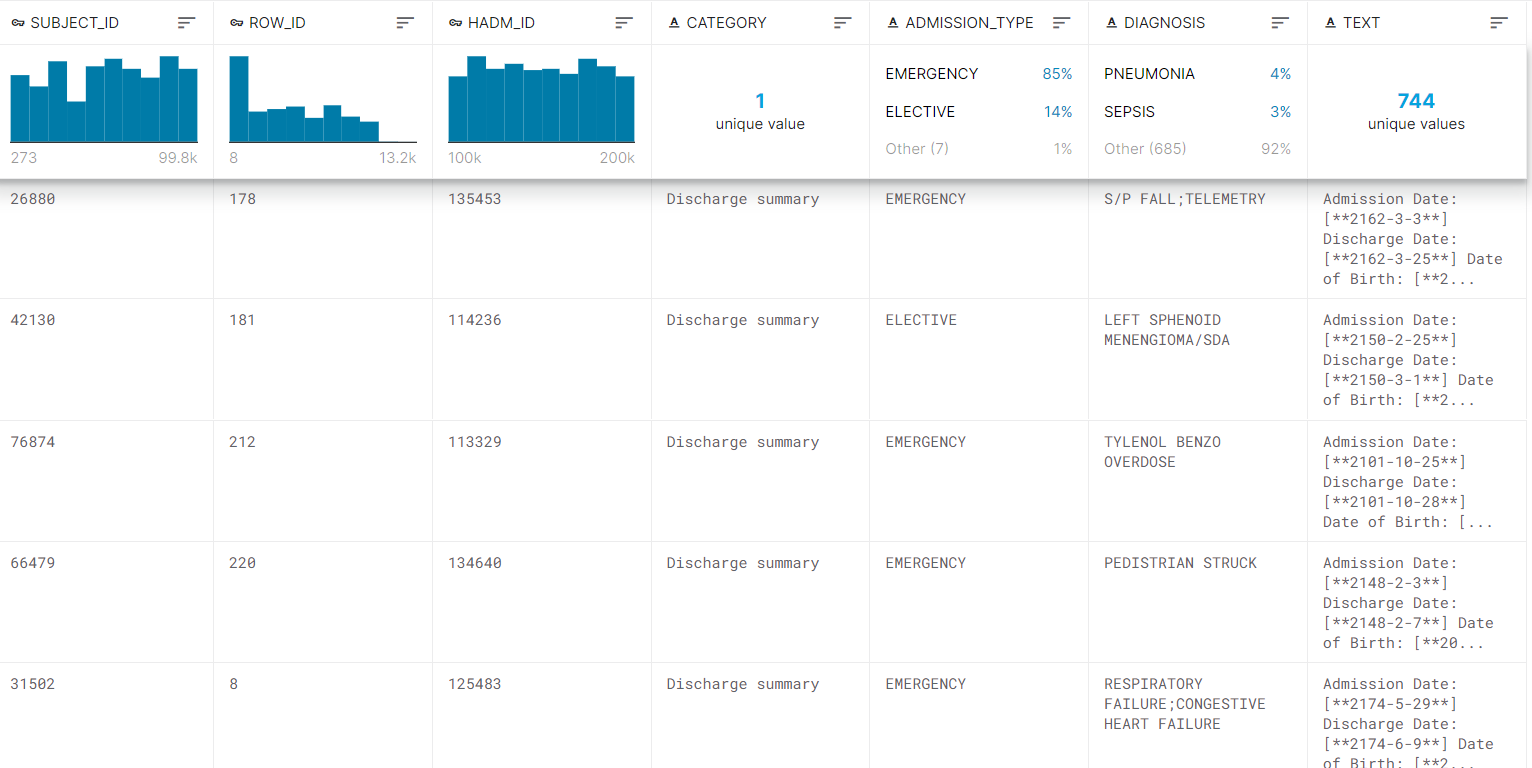
\includegraphics[width=0.65\textwidth]{images/chapter3/dataset/healthprescription.PNG}
    \caption{A sample of Health Prescription dataset.}
    \label{fig:presc}
  \end{figure}
  \item We have collected a collection of x-ray images and other images type.
  \newpage
  \item \textbf{Liver Patient Records Dataset:} This data set contains liver and non-liver patient records collected from North East of Andhra Pradesh, India. The dataset contains the age and the gender of the patient, Total Bilirubin, Direct Bilirubin, Alkaline Phosphatase and others (Figure\ref{fig:liver}).
  \begin{figure}[h!]
    \center
    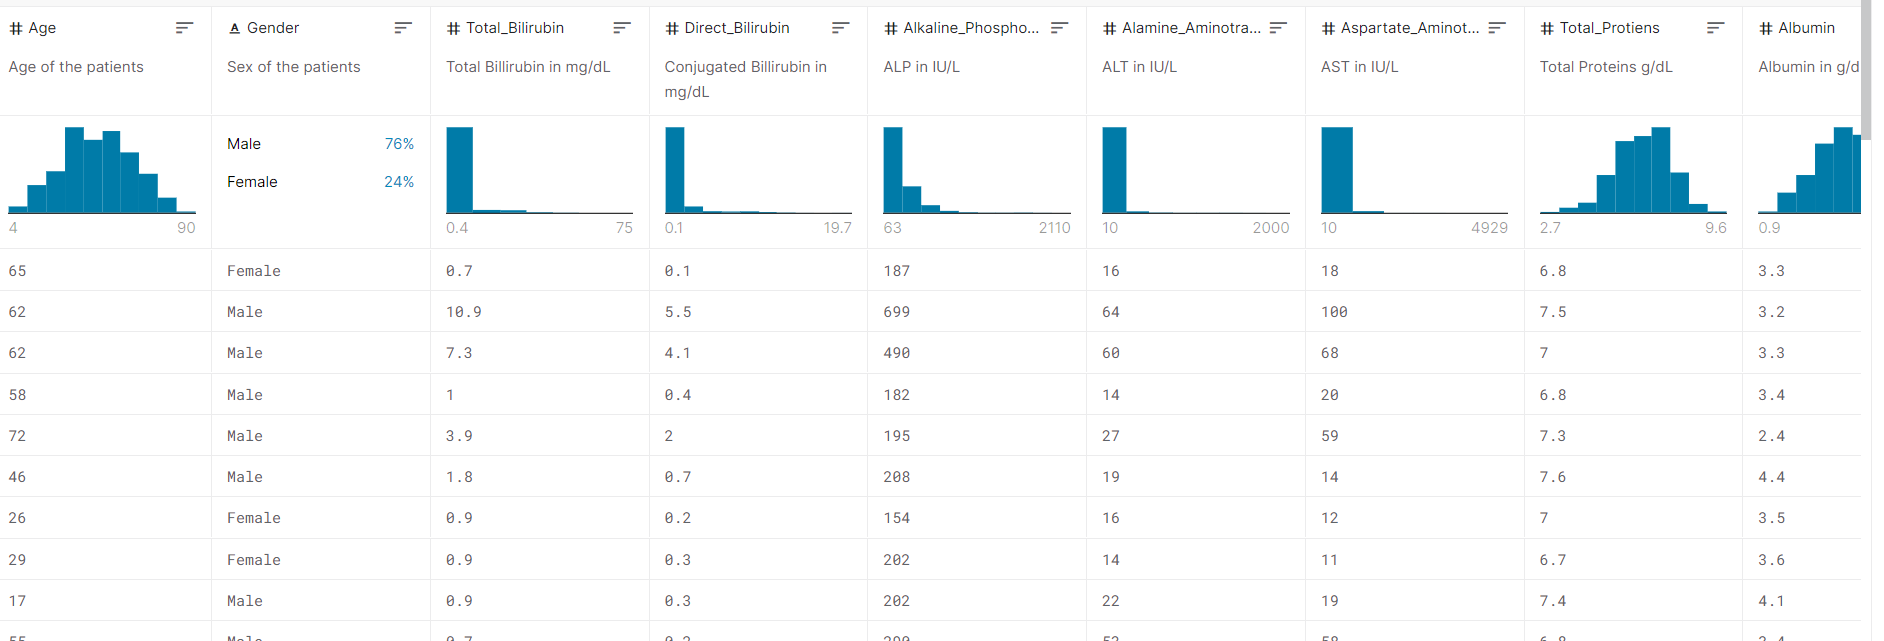
\includegraphics[width=0.65\textwidth]{images/chapter3/dataset/indianliver.PNG}
    \caption{A sample of Liver Patient Records dataset.}
    \label{fig:liver}
  \end{figure}
  \item \textbf{Disease Symptom Prediction Dataset:} There are columns containing diseases, their symptoms , precautions to be taken, and their weights (Figure\ref{fig:simptoms}).
  \begin{figure}[h!]
    \center
    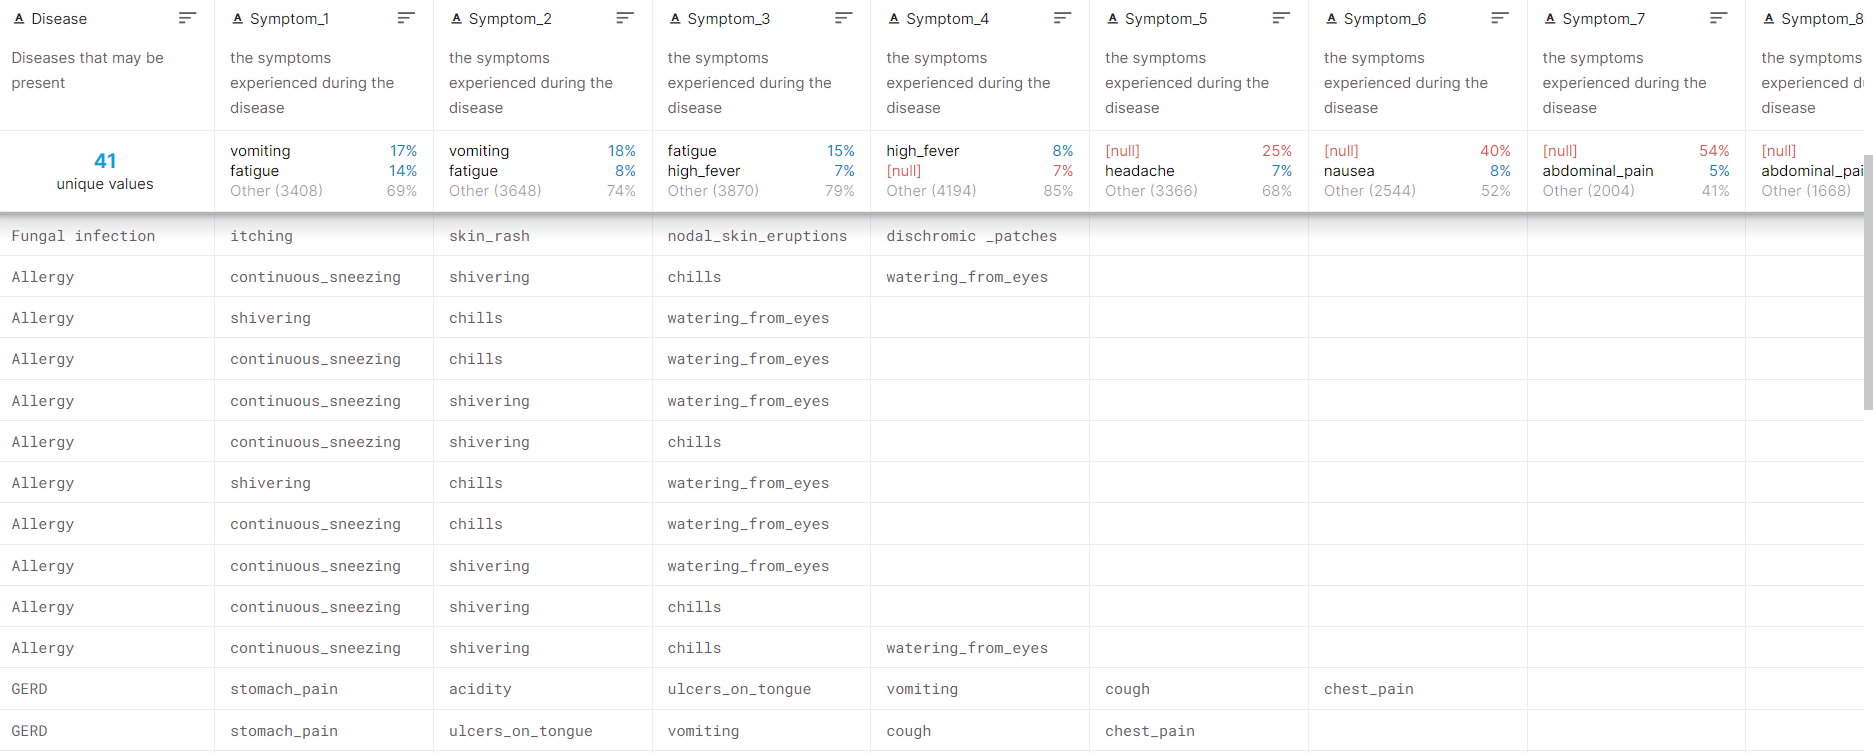
\includegraphics[width=0.65\textwidth]{images/chapter3/dataset/simptoms.PNG}
    \caption{A sample of Disease Symptom Prediction dataset.}
    \label{fig:simptoms}
  \end{figure}
  \item \textbf{Patient Treatment Classification:} This dataset is Electronic Health Record Predicting collected from a private Hospital in Indonesia. It contains the patient's laboratory test results: name, data type, value sample, description (Figure\ref{fig:treat}).
  \begin{figure}[h!]
    \center
    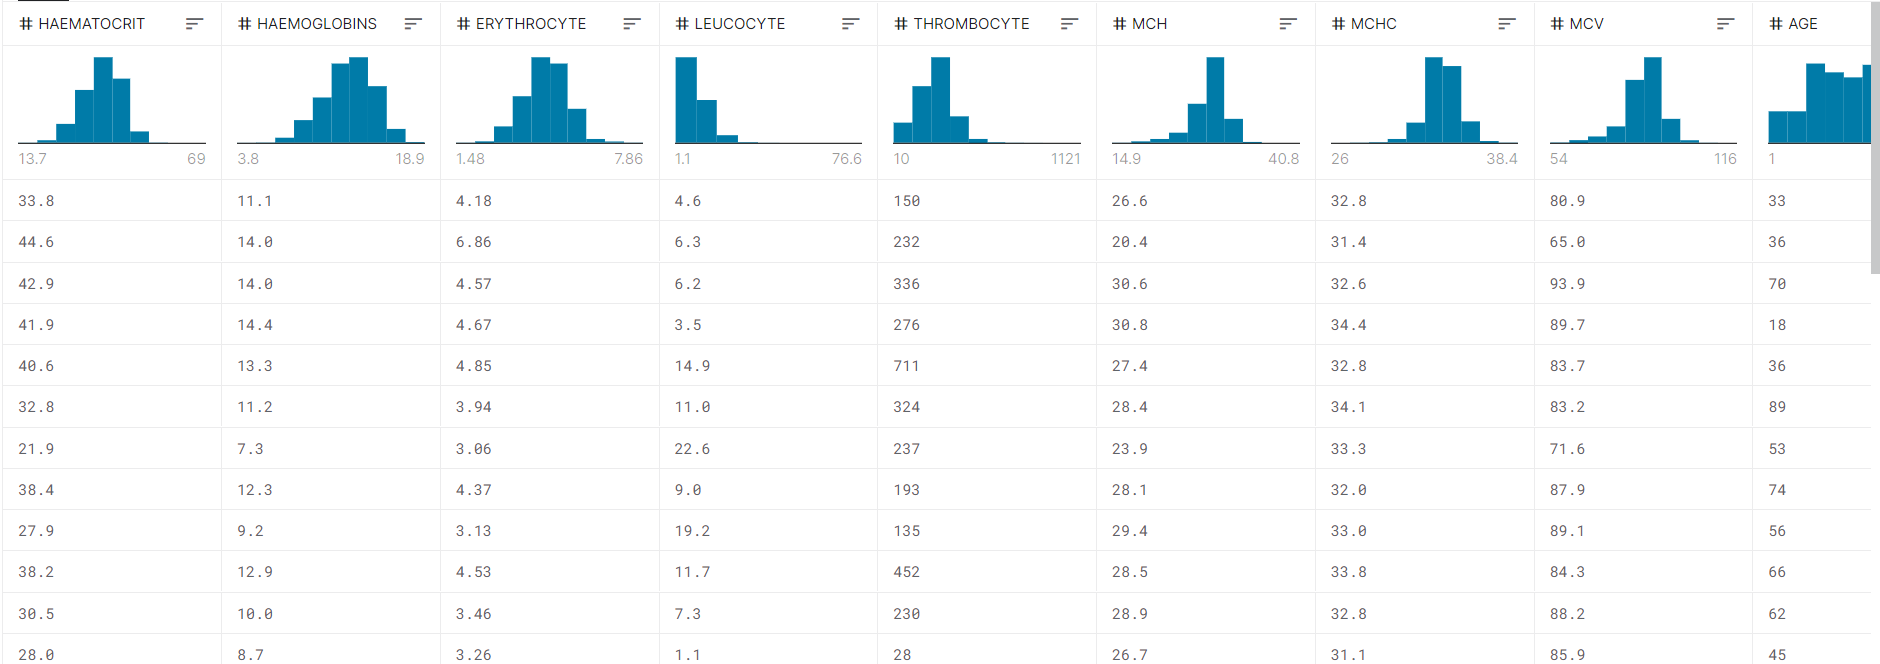
\includegraphics[width=0.65\textwidth]{images/chapter3/dataset/treat.PNG}
    \caption{A sample of Patient Treatment Classification dataset.}
    \label{fig:treat}
  \end{figure}
  
  \end{itemize}
  
\subsubsection*{Pretreatment}
We wanted to present the entered data as if it comes from several medical actors, for this we created a fake data based on the dataset collected before, using python libraries (\ref{sec:python}) to present the patients information, their lab test results, their diagnosis etc.


\begin{figure}[h!]
  \begin{subfigure}{.60\textwidth}
      \center
      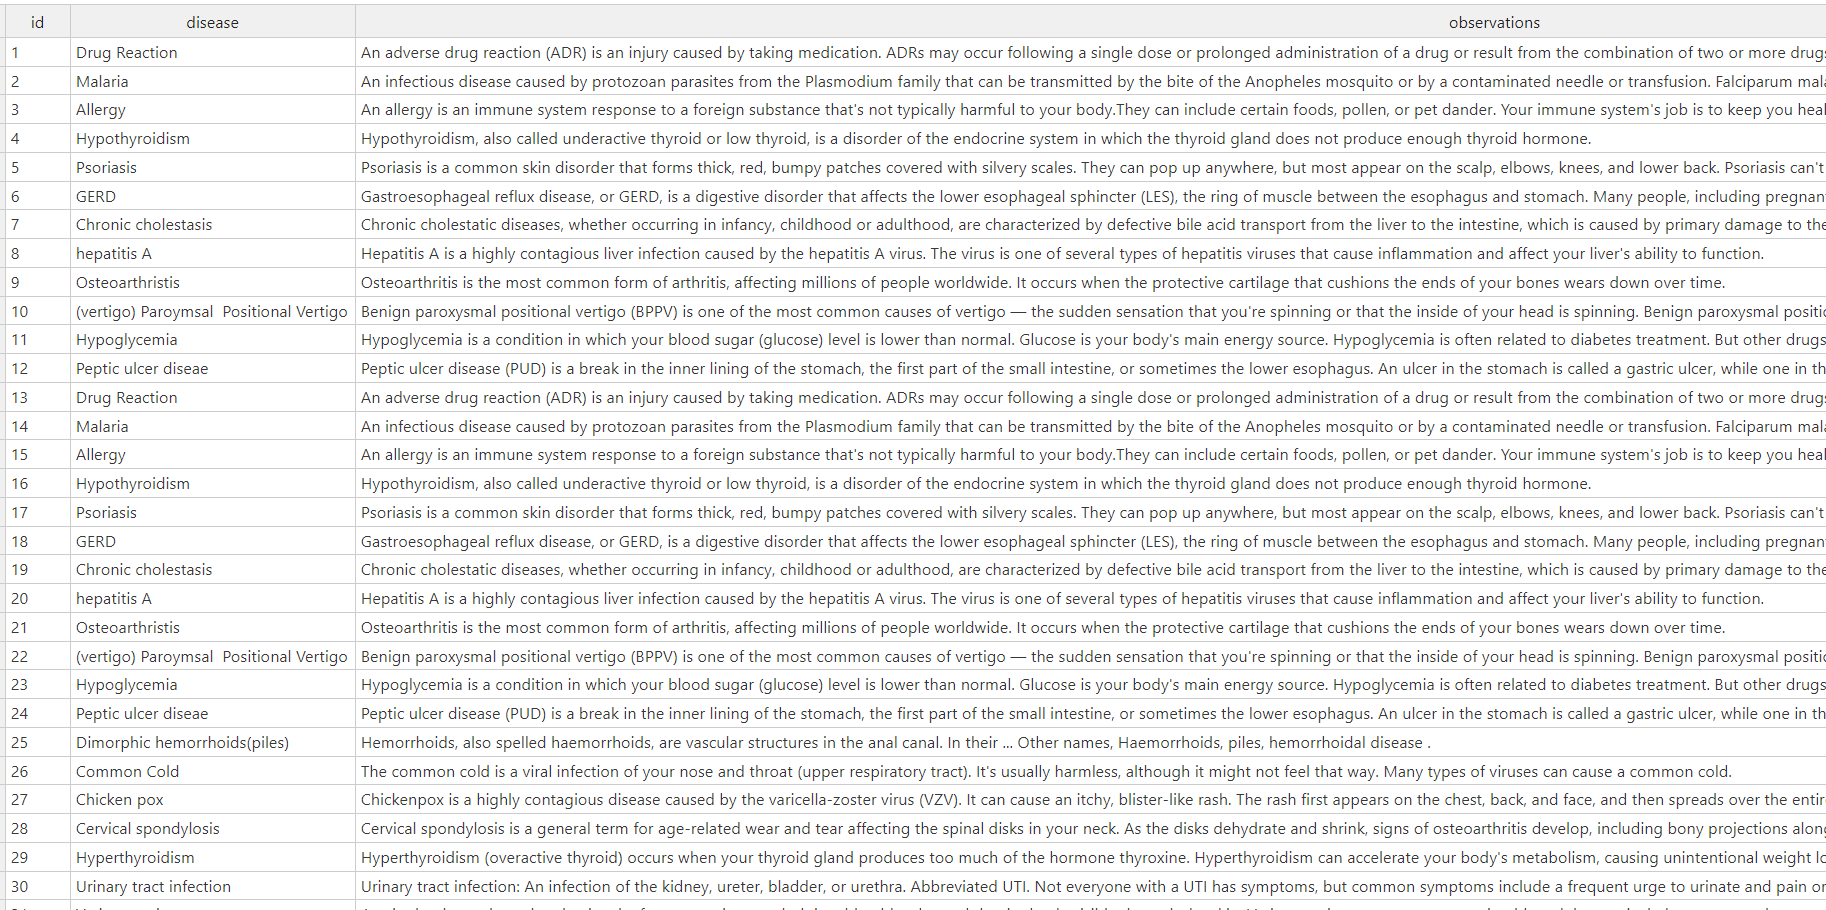
\includegraphics[width=0.95\textwidth]{images/chapter3/pretartmntData/diagnosis.PNG}
  \end{subfigure}
  \begin{subfigure}{.60\textwidth}
    \center
    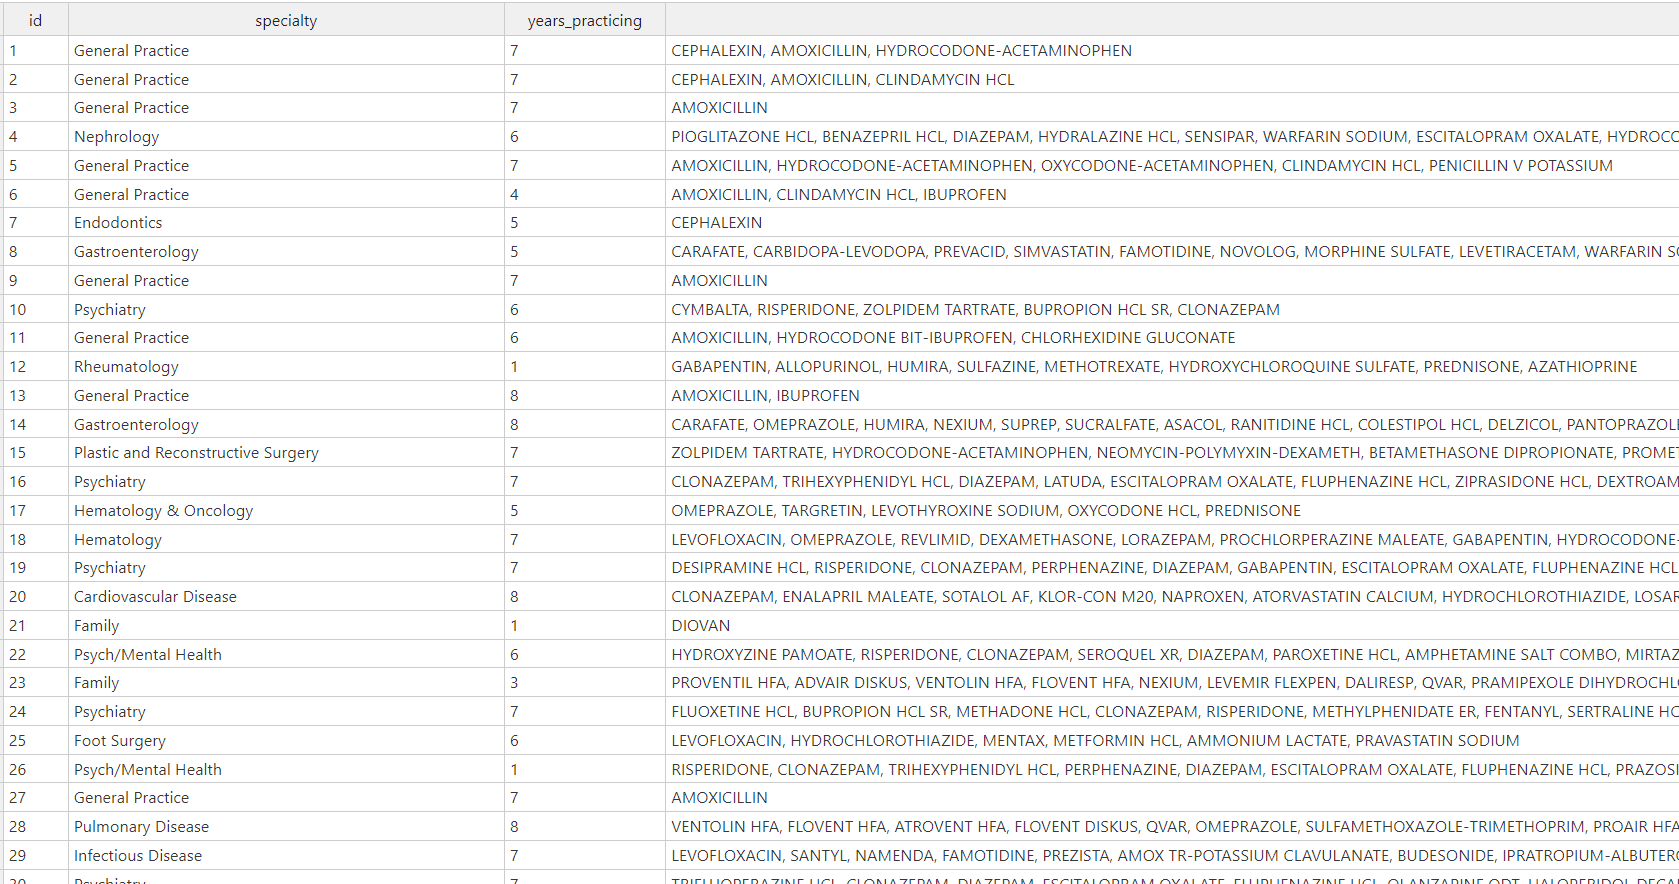
\includegraphics[width=0.95\textwidth]{images/chapter3/pretartmntData/medicalrecord.PNG}
    
\end{subfigure}
\caption{Samples of our data after the pretreatment.}
\end{figure}




\begin{figure}[h!]
  \begin{subfigure}{.55\textwidth}
      \center
      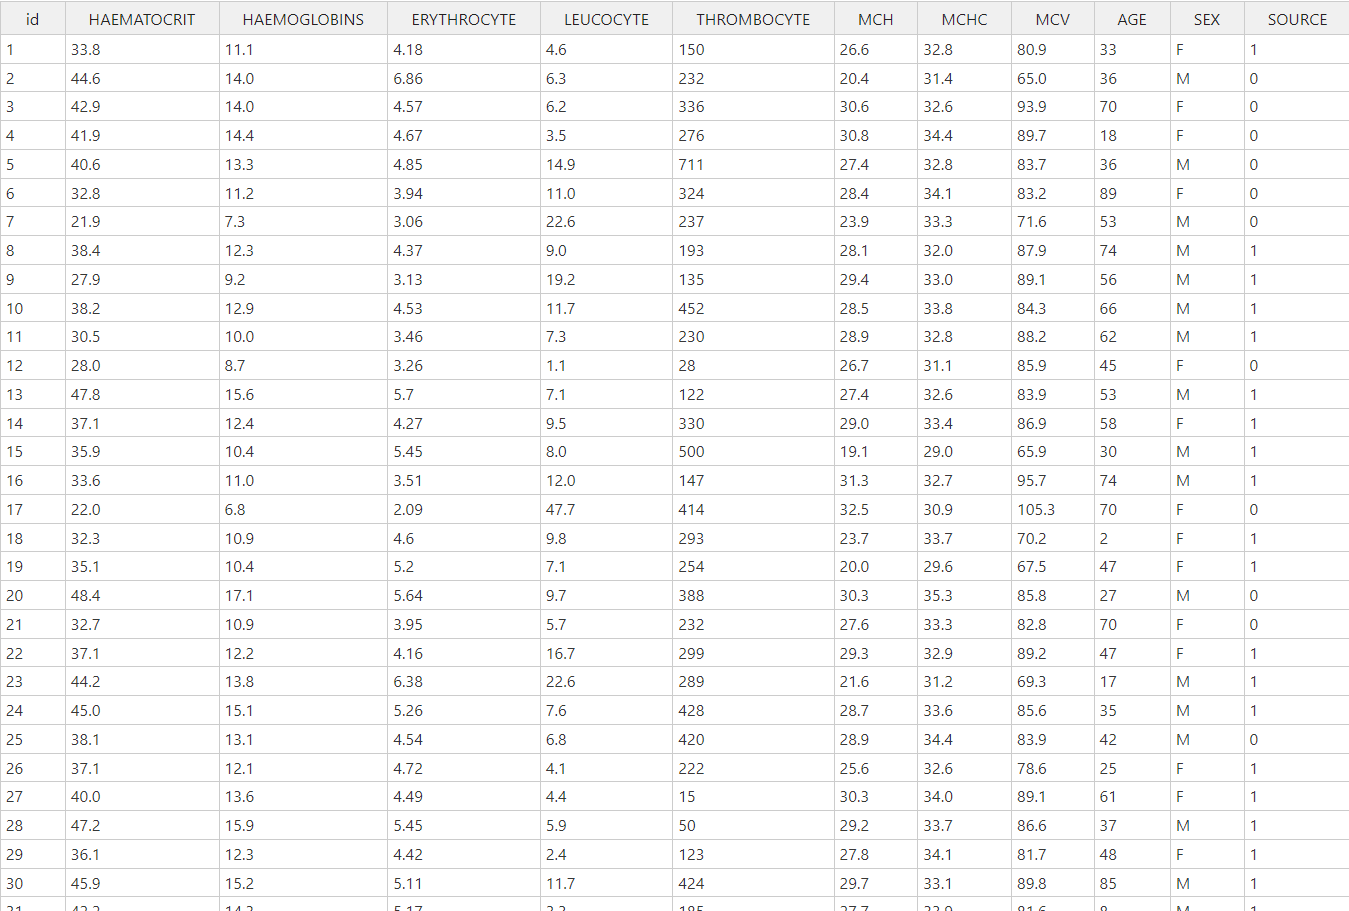
\includegraphics[width=0.95\textwidth]{images/chapter3/pretartmntData/labtests.PNG}
  \end{subfigure}
  \begin{subfigure}{.55\textwidth}
    \center
    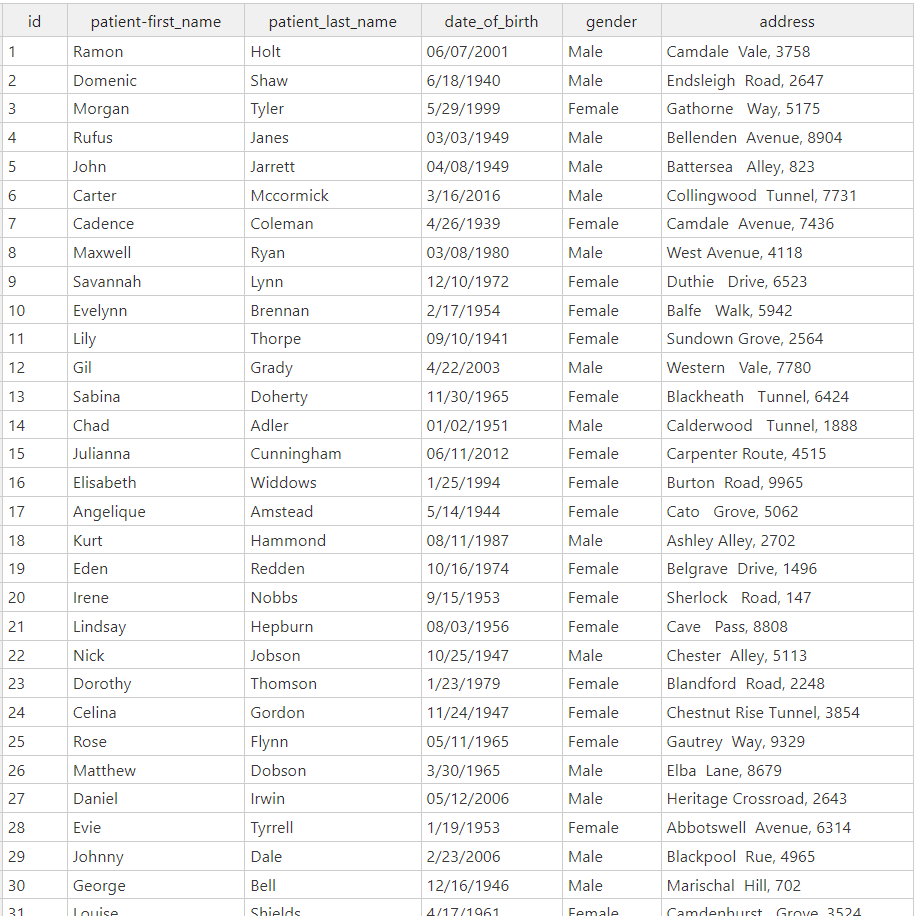
\includegraphics[width=0.90\textwidth]{images/chapter3/pretartmntData/patientInfo.PNG}
    
\end{subfigure}
  
  \caption{Samples of our data after the pretreatment.}
  
\end{figure}

\newpage

\subsubsection*{Data Integration \& Treatment}


After the data was collected and pre-processed, we integrated it using Talend open studio (\ref{sec:talend}), the input data was the pretreated data we introduced it in the previous section, each entry represent an medical source, we used Talend tmap component to build our output data.

\begin{figure}[h!]
  \center
  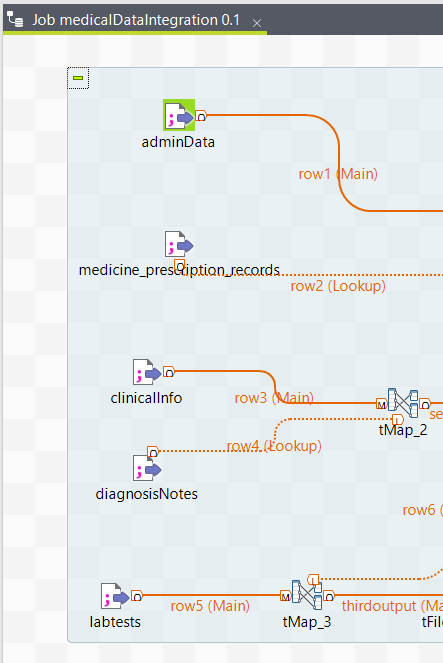
\includegraphics[width=0.40\textwidth]{images/chapter3/jobInputs.PNG}
  \caption{Input data.}
  \label{fig:jobinputes}
\end{figure}
\begin{figure}[h!]
  \center
  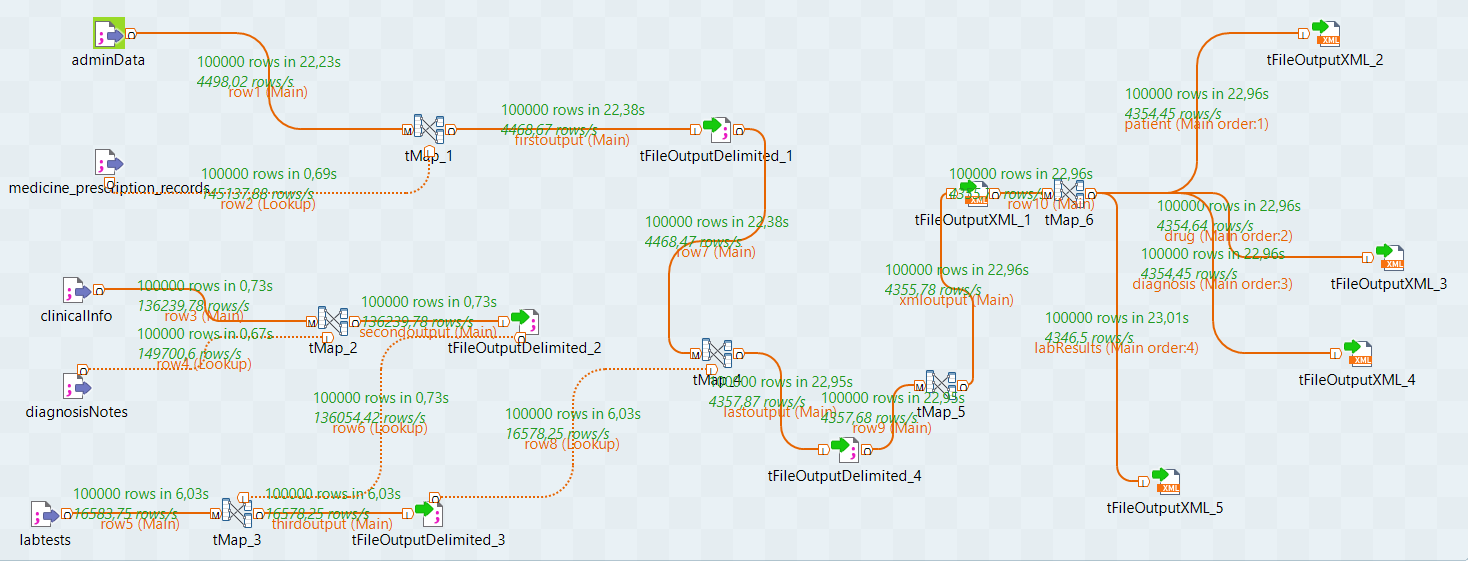
\includegraphics[width=0.80\textwidth]{images/chapter3/jobresult.PNG}
  \caption{Talend job execution.}
  \label{fig:jobtalend}
\end{figure}
\newpage
\subsubsection*{Output Data}
Our main objective was to extract the following data (each head represents an XML node):
\begin{figure}[h!]
  \center
  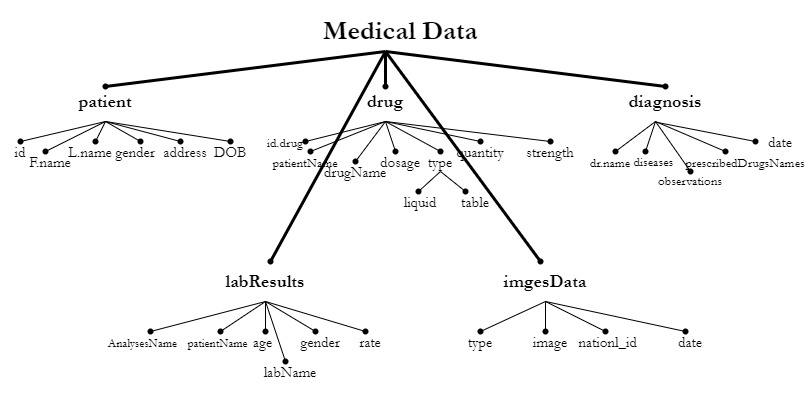
\includegraphics[width=0.99\textwidth]{images/chapter3/tree.jpg}
  \caption{The corresponding tree of XML schema.}
  \label{fig:xmlschema}
\end{figure}
\begin{itemize}
\renewcommand{\labelitemi}{$\bullet$}
\item \textbf{Patient:} That presents the administrative information about the patient x, including his full name, national ID, gender, date of birth, address. 
\item \textbf{Drug:} Presents the list of drugs in the patient’s  prescription, it includes: the drug’s name, its dosage, strength usually mentioned by the doctor, the quantity, and its type(liquid or table).
\item \textbf{Diagnosis:} Includes the doctor's name, the diseases name, and the observations taken by the medical actor in charge, it also contains the patient’s national ID, the name of the prescribed medications and the date of diagnosis. 
\item \textbf{LabResults:} It presents the medical biology results that includes the analysis’s name, the patient rate saved, the gender and the age for the comparison (a predefined high/low rate is defined corresponding to each analysis), attached with the laboratory name and the patient's national ID.
\item \textbf{ImagesData:} Present the data of the image obtained by the patient, it includes the image name and the image itself, the day it was taken, and the patient's national ID.
\end{itemize}

\bigbreak
The resulting data will be used as a source to feed all the components of the digital marketing reporting applications that are built in many visualization tools(\ref{sec:tool}).

\subsection{Data Rendering}

Once the xml output data is prepared, the data rendering phase is started, it consists of 3 stages as illustrated in the following figure:

\begin{figure}[h!]
  \center
  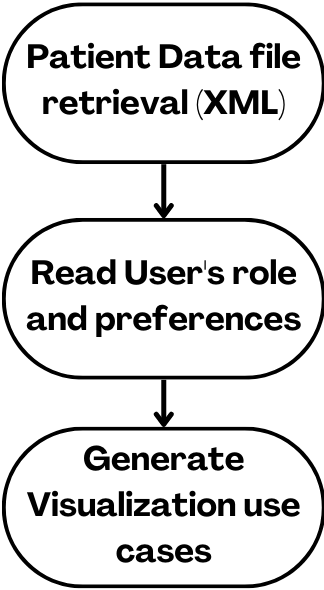
\includegraphics[width=0.20\textwidth]{images/chapter3/rendering.png}
  \caption{The data rendering flowchart.}
  \label{fig:rendering}
\end{figure}

\subsubsection*{Patient Data file retrieval (XML)}
This step consists of integrating the XML files into the visualization script. In our project process, we generated 4 files that revolve around the patient record and integrated them:
\begin{itemize}
  \renewcommand{\labelitemi}{$\bullet$}
  \item \textbf{patient.xml: }Contains patient information.
  \item \textbf{diagnostic.xml: }Contains the patient's diagnosis.
  \item \textbf{drug.xml: }Contains the drugs prescribed to the patient.
  \item \textbf{labResults.xml: }Contains patient lab test results.
\end{itemize}

\subsubsection*{Read User's role and preferences}
This step consists of analyzing the user's role and need in order to display the appropriate visualization graphs. For this project, we have created three predefined users: the patient, the doctor, and the administrator, each one has his own preferences.\\
The data will be displayed according to that.
\newpage
\subsubsection*{Generate Visualization use cases}
For the purpose of generating the appropriate graphs we needed to go through several analyzing steps:
\begin{itemize}
\renewcommand{\labelitemi}{$\bullet$}
\item Analyzing the input data usually depends on the data properties.
\item Analyzing the data type (quantitative (continuous or Discrete quantitative) or qualitative (ordinal or nominal)).
\item The questions to be answered.
\item How the information should be presented.
\item The size of the dataset.
\item And the audience (actors).
\end{itemize}

\bigbreak
Depending on the libraries we integrated in this project, we used different types of graphs to present the quantitative data, each based on the factor mentioned previously and the frequent questions asked from our point of view.
\begin{itemize}
  \renewcommand{\labelitemi}{$\bullet$}
  \item To express comparison between parts of a bigger set of data, highlighting different categories, or showing change over time, we used: bar charts type.
  \item To show relative proportions and percentages of a whole dataset or to compare the effect of ONE factor on different categories or to express nominal and not ordinal data, we used: pie charts type. 
  \item To express a continuous dataset that changes over time or to display multiple series for the same timeline or to visualize trends instead of exact values, we used: line charts type.
\item To show correlation and clustering in big datasets or the dataset containing points that have a pair of values, we used: Scatter Plot type.
\end{itemize}


\begin{figure}[h!]
  \begin{subfigure}{.50\textwidth}
      \center
      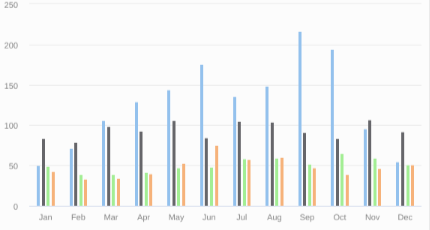
\includegraphics[width=0.50\textwidth]{images/chapter3/chartexmple/bar.PNG}
      \caption{Bar chart.}
  \end{subfigure}
  \begin{subfigure}{.50\textwidth}
      \center
      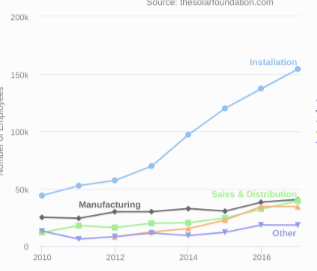
\includegraphics[width=0.50\textwidth]{images/chapter3/chartexmple/line.PNG}
      \caption{Line chart.}
  \end{subfigure}
  \begin{subfigure}{.50\textwidth}
      \center
      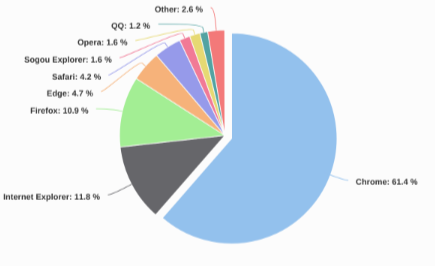
\includegraphics[width=0.50\textwidth]{images/chapter3/chartexmple/pie.PNG}
      \caption{Pie chart.}
  \end{subfigure}
  \begin{subfigure}{.50\textwidth}
      \center
      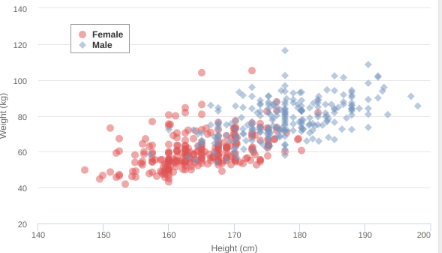
\includegraphics[width=0.50\textwidth]{images/chapter3/chartexmple/scatter.PNG}
      \caption{Scatter plot.}
  \end{subfigure}
  \caption{The different used charts.}
\end{figure}
\newpage
\subsection{Image Data}
The rendering data produced from the previous phase will be displayed in  personalized dashboard in the next chapter.
%TODO: add ref to the chapter
\section{Conclusion}
In this chapter, we presented the proposed system process, which goes through three phases: data preparation, data rendering, Image data. The data preparation phase consists of choosing the row data and pretreating it then integrating it. The data rendering phase consists of analyze the output data to display it in the last next phase,  this phase consists of three stages:  Patient Data file retrieval (XML), Read User’s role and preferences, then Generate Visualization use cases , and lastly the image data phase that will be explained in the next chapter. 
